% !TeX encoding=utf8
% !TeX spellcheck = de_DE
% !TeX root = ../Diploma.tex

\chapter{Konzept des Clients}\label{sec:conceptClient}
In diesem Kapitel ist die Konzeption des Schachclients, welche die Grundlage für die Umsetzung selbigem bildet. Dabei werden im ersten Abschnitt die benötigten Anforderungen beschrieben, die der Client erfüllen muss. Im zweiten Abschnitt erfolgt die Visualisierung und Beschreibung der einzelnen Ansichten, welche für eine bequeme Nutzerinteraktion benötigt werden.

\section{Anforderungen}\label{sec:anforderungenClient}
Grundlegend soll der Client als Visualisierung des Servers dienen. Dafür ist eine Verwaltung von Playern und Matches bereitzustellen, inklusive der Möglichkeit zum Anlegen neuer bzw. Bearbeiten schon angelegter Einträge. Um anschließend auch Schach spielen zu können, muss der Client dafür eine komfortable Möglichkeit in Form eines virtuellen Schachbrettes bieten.\\
\\
Als Grundanforderung dafür muss der Client natürlich mit dem Server kommunizieren können. Dafür muss dieser Requests senden und die empfangenen Response-Nachrichten verarbeiten können. Da der Server für manche Request spezielle Parameter benötigt, wie zum Beispiel einen String in der \gls{SAN}, müssen diese gegebenenfalls ermittelt werden können.\\
\\
Für ein bequemes Spielerlebnis soll der Client ein gestartetes Match automatisch aktualisieren, sobald sich die Daten auf dem Server verändert haben. Um dies zu realisieren, ist ein einfaches Polling-Verfahren zu implementieren.\\
\\ 
Die letzte Grundanforderung ist eine innovative und benutzerfreundliche Bedienung der Anwendung, so dass der Nutzer keinerlei Kenntnisse außer den Schachregeln besitzen muss.

\section{Mockups der Client-Ansichten}\label{sec:views}
In diesem Abschnitt wird auf Basis der im Kapitel 5.1\hyperref[sec:anforderungenClient]{Kapitel~\ref{sec:anforderungenClient}} definierten Anforderungen ein Konzept entwickelt. Ziel ist dabei die Erstellung von Mockups der einzelnen Ansichten, um die Implementierung zu vereinfachen bzw. zu beschleunigen.

\subsection{Startansicht}\label{sec:startView}
Die Startansicht ist der Ausgangspunkt für die Nutzer, welche beim Aufruf der Root-\gls{URL} zurückzugeben ist. Mithilfe der Startansicht soll dem Nutzer die Möglichkeit bereitgestellt werden zur Player-Ansicht bzw. zur Match-Ansicht zu wechseln. Dafür ist ihm jeweils ein Button zum Auslösen dieses Wechsels zur Verfügung zustellen.\\
\\
Die \hyperref[fig:startView]{Abbildung~\ref{fig:startView}} visualisiert dabei die zuvor definierten Anhaltspunkte der Startansicht.
\begin{figure}[htb]
	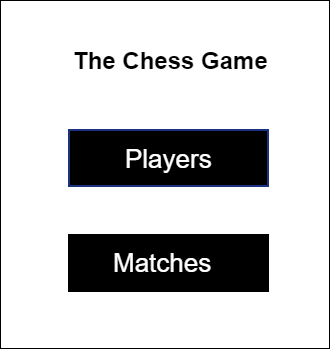
\includegraphics[width=0.234\textwidth]{images/start-view.png}
	\caption{Mockup: Startansicht des Clients}
	\label{fig:startView}
\end{figure}

\subsection{Player-Ansicht}\label{sec:playerView}
Mit dieser Ansicht ist dem Nutzer die Möglichkeit bereitzustellen, alle angelegten Player zu verwalten. Dafür muss ihm eine Tabelle für die Übersicht und ein Formular zum Anlegen neuer oder Bearbeiten bereits angelegter Player bereitgestellt werden. Über eine Spalte innerhalb der Tabelle sollen Buttons zur Verfügung stehen, über welche ein Player bearbeitet oder gelöscht werden kann.\\
\\
Aus diesen ermittelten Punkten wurde das Mockup aus der \hyperref[fig:playerView]{Abbildung~\ref{fig:playerView}} entworfen, um diese visuell hervorzuheben.
\begin{figure}[htb]
	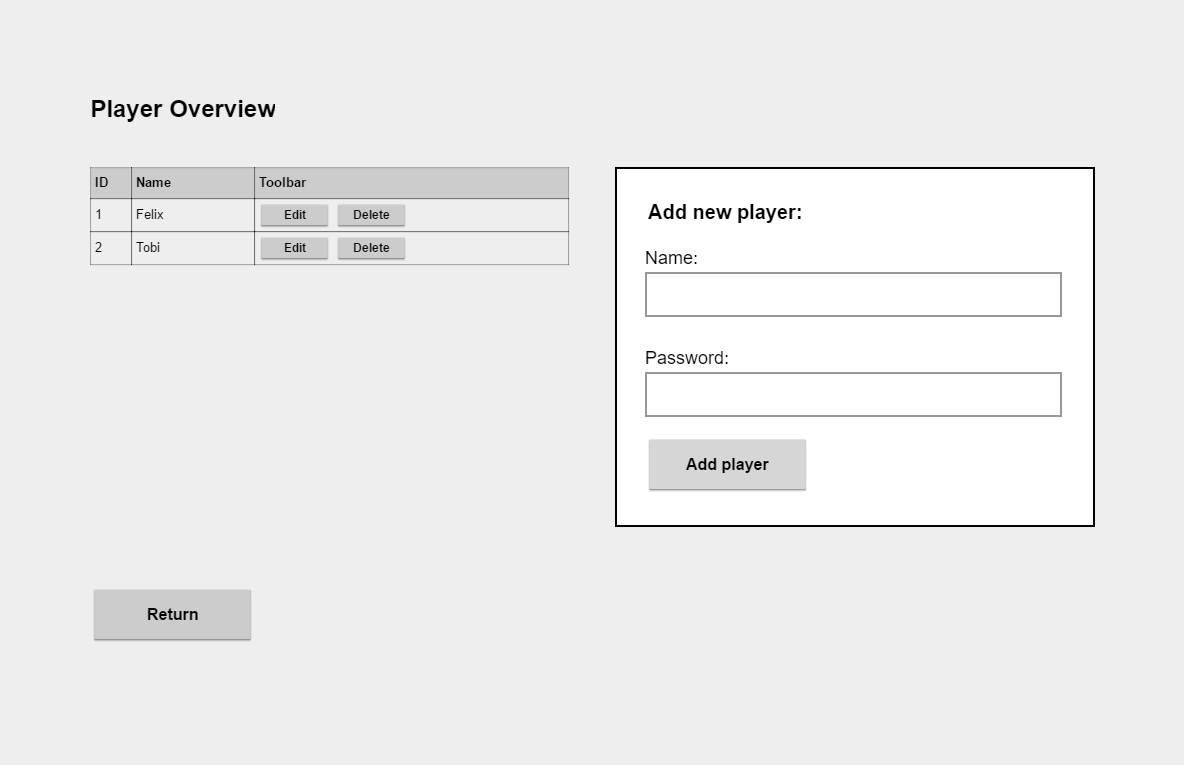
\includegraphics[width=0.84\textwidth]{images/player-view.png}
	\caption{Mockup: Player-Ansicht des Clients}
	\label{fig:playerView}
\end{figure}

\subsection{Match-Ansicht}\label{sec:matchView}
Mithilfe der Match-Ansicht ist dem Nutzer eine Match-Verwaltung zur Verfügung zustellen. Um dabei die Konsistenz zu wahren, ist auch diese genau so aufgebaut wie die Player-Ansicht, mit dem Unterschied, dass ein Match nicht gelöscht aber dafür gestartet werden kann. Daher ändern sich geringfügig die Buttons in der Tabelle.\\
\\
Dabei werden die gefundenen Fakten durch die \hyperref[fig:matchView]{Abbildung~\ref{fig:matchView}} grafisch dargestellt.
\begin{figure}[htb]
	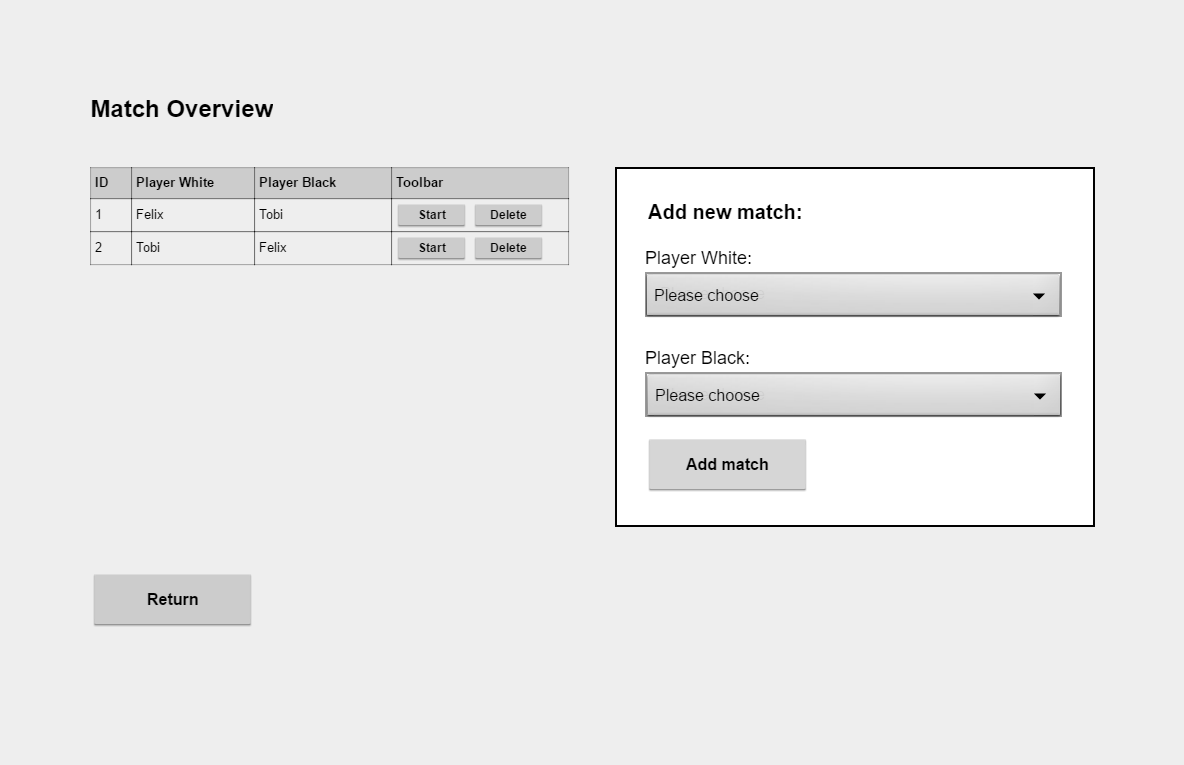
\includegraphics[width=0.84\textwidth]{images/match-view.png}
	\caption{Mockup: Match-Ansicht des Clients}
	\label{fig:matchView}
\end{figure}

\subsection{Ansicht eines gestarteten Matches}\label{sec:gameView}
Mithilfe dieser Ansicht soll dem Nutzer ermöglicht werden ein gestartetes Match zu spielen. Dafür wird in erster Linie ein Schachbrett benötigt, auf welchem die Figuren dargestellt werden. Mittels \enquote{Drag \& Drop} soll der Nutzer anschließend Spielfiguren bewegen können. Für eine einfachere Bedienung und zur Unterstützung des Verständnisses der Schachregeln sollen alle möglichen Züge einer Figur hervorgehoben werden, sobald über diese mit der Maus gefahren wird. Da Informationen über bereits geschmissene Figuren oder welche Züge bisher getätigt wurden sehr hilfreich sein können, sollen diese neben dem Schachbrett dargestellt werden. \\
\\
Anhand dieser Kriterien an die Ansicht eines gestarteten Matches wurde das Mockup aus der \hyperref[fig:gameView]{Abbildung~\ref{fig:gameView}} entwickelt.\\
\begin{figure}[htb]
	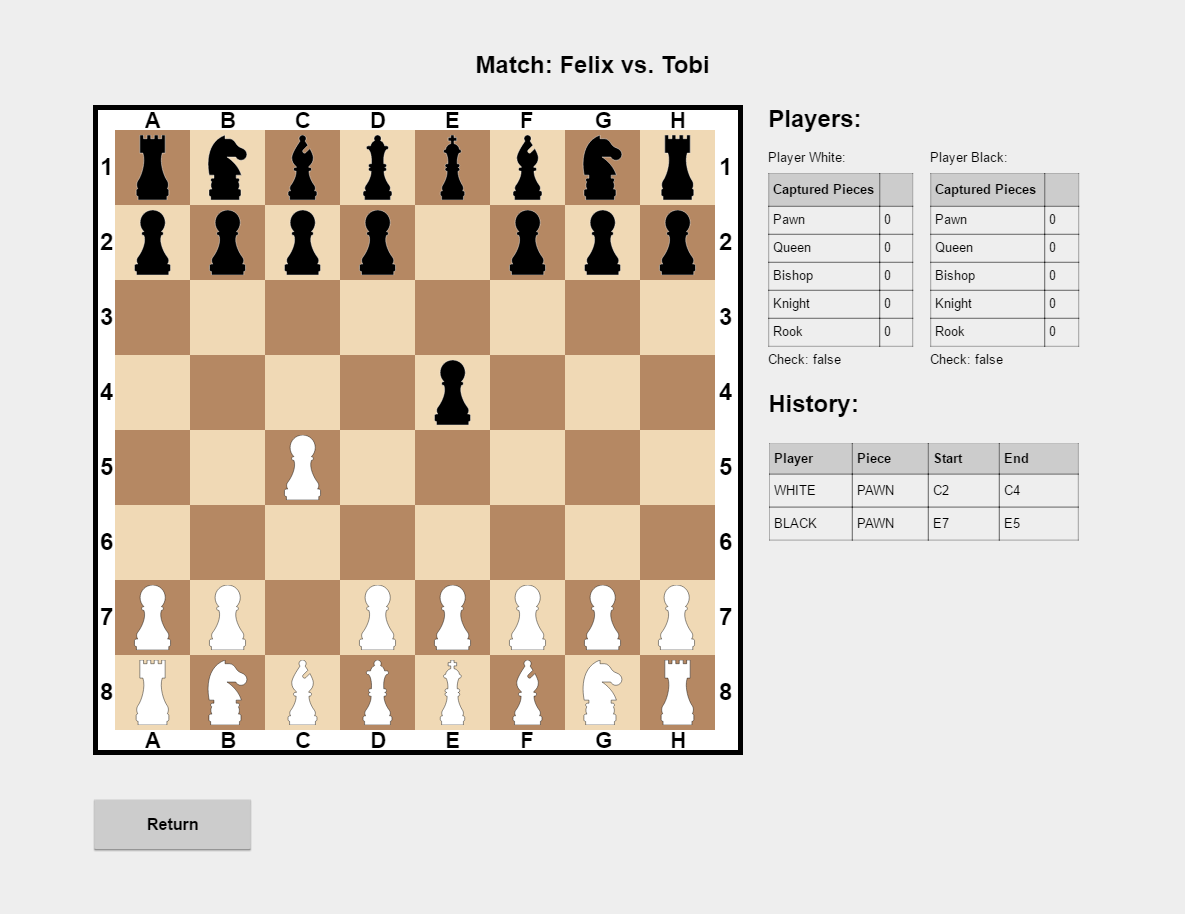
\includegraphics[width=0.84\textwidth]{images/game-view.png}
	\caption{Mockup: Ansicht eines gestarteten Matches}
	\label{fig:gameView}
\end{figure}


